\documentclass[a4 paper]{article}
\usepackage{xcolor}
\usepackage{graphicx}

\title{HW-3 / REPORT}

\author{ Can Duyar - 171044075}

\begin{document}
\date{}
\maketitle

{\color{red}\large\textbf {Solving The Problem And Design Decisions:}}\newline\\
\textbf{Checking arguments and identify them:} We need 8 arguments in this program. And there will be an another argument program running
command. So, we will have total 9 arguments. If total arguments less than 9 then print right format for running this program and finish the program.\newline\\
\textbf{Reading arguments:} Check argument identifiers and based on argument identifiers assign arguments as potato
counts, shared memory name, shared semaphore name, and FIFO name containing file. After that the program will check every required argument is given or not, if every required argument is not given then show error message and finish program.\newline\\
\textbf{Shared memory:} Mapping shared memory by given name. This memory will have used to shared common data.Like: shared memory is initialized or not, total turns to cooled down potato, committed turns,sender’s information, sharing semaphore’s state, FIFO name pickup, and potato number.\newline\\
\textbf{Semaphore:} Get shared named semaphore. This semaphore will be used for synchronization. While player will not ready for reading pipe it will lock the semaphore. Sender player will check every receiver player is ready or not through semaphore. If everyone is ready, then it will send the potato to a random FIFO.\newline\\
\textbf{FIFO names from file:} It will open the given file to read FIFO names. It will read a name at a time and will check this name is taken or not. If name isn’t taken, then it will take that as its FIFO name. Else it will store that name into a variable to pick up randomly while it will send the potato to another player.\newline\\
\textbf{Potatoes:} Program will check potato is given to it or not. If given, then it assigns the potato number and total turns to cooled down the potato. After that it will check all receiver players are ready or not. If not ready, then it will wait or else it will send the potato to a random FIFO pipe. Here it will use the semaphore for waiting until everyone is ready.\newline\\
\textbf{Receive message:} Every initialization is finished so, now player will wait for potato through its pipe. When player get a potato through pipe it will show the message and check if the potato is cooled down or not using shared date from shared memory. If cooled down, then show message and it goes to wait again for another potato. Else it will update shared data in shared memory and send potato to a random FIFO pipe after checking every receiver is ready using semaphore. And then it goes to wait again for another potato. When player get a terminate message through pipe it simply free up all allocated memory and finish the program.\newline\\
\textbf{Signal to terminate:} When any player gets a signal (Ctrl+C) to terminate the program then it will send a terminate message to all active player through pipe and then free up allocated memory and finish program.\newline\\
\textbf{Note:} There is no possible memory leaks in my code. I checked it with valgrind. also there is no zombie processes.\newline\\

\begin{figure}[ht!]
	\centering
	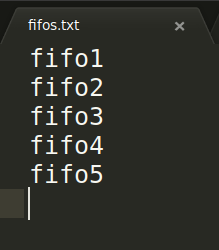
\includegraphics[width=20mm]{1.png}
	\caption{example: fifos.txt \label{overflow}}
\end{figure}

\begin{figure}[ht!]
	\centering
	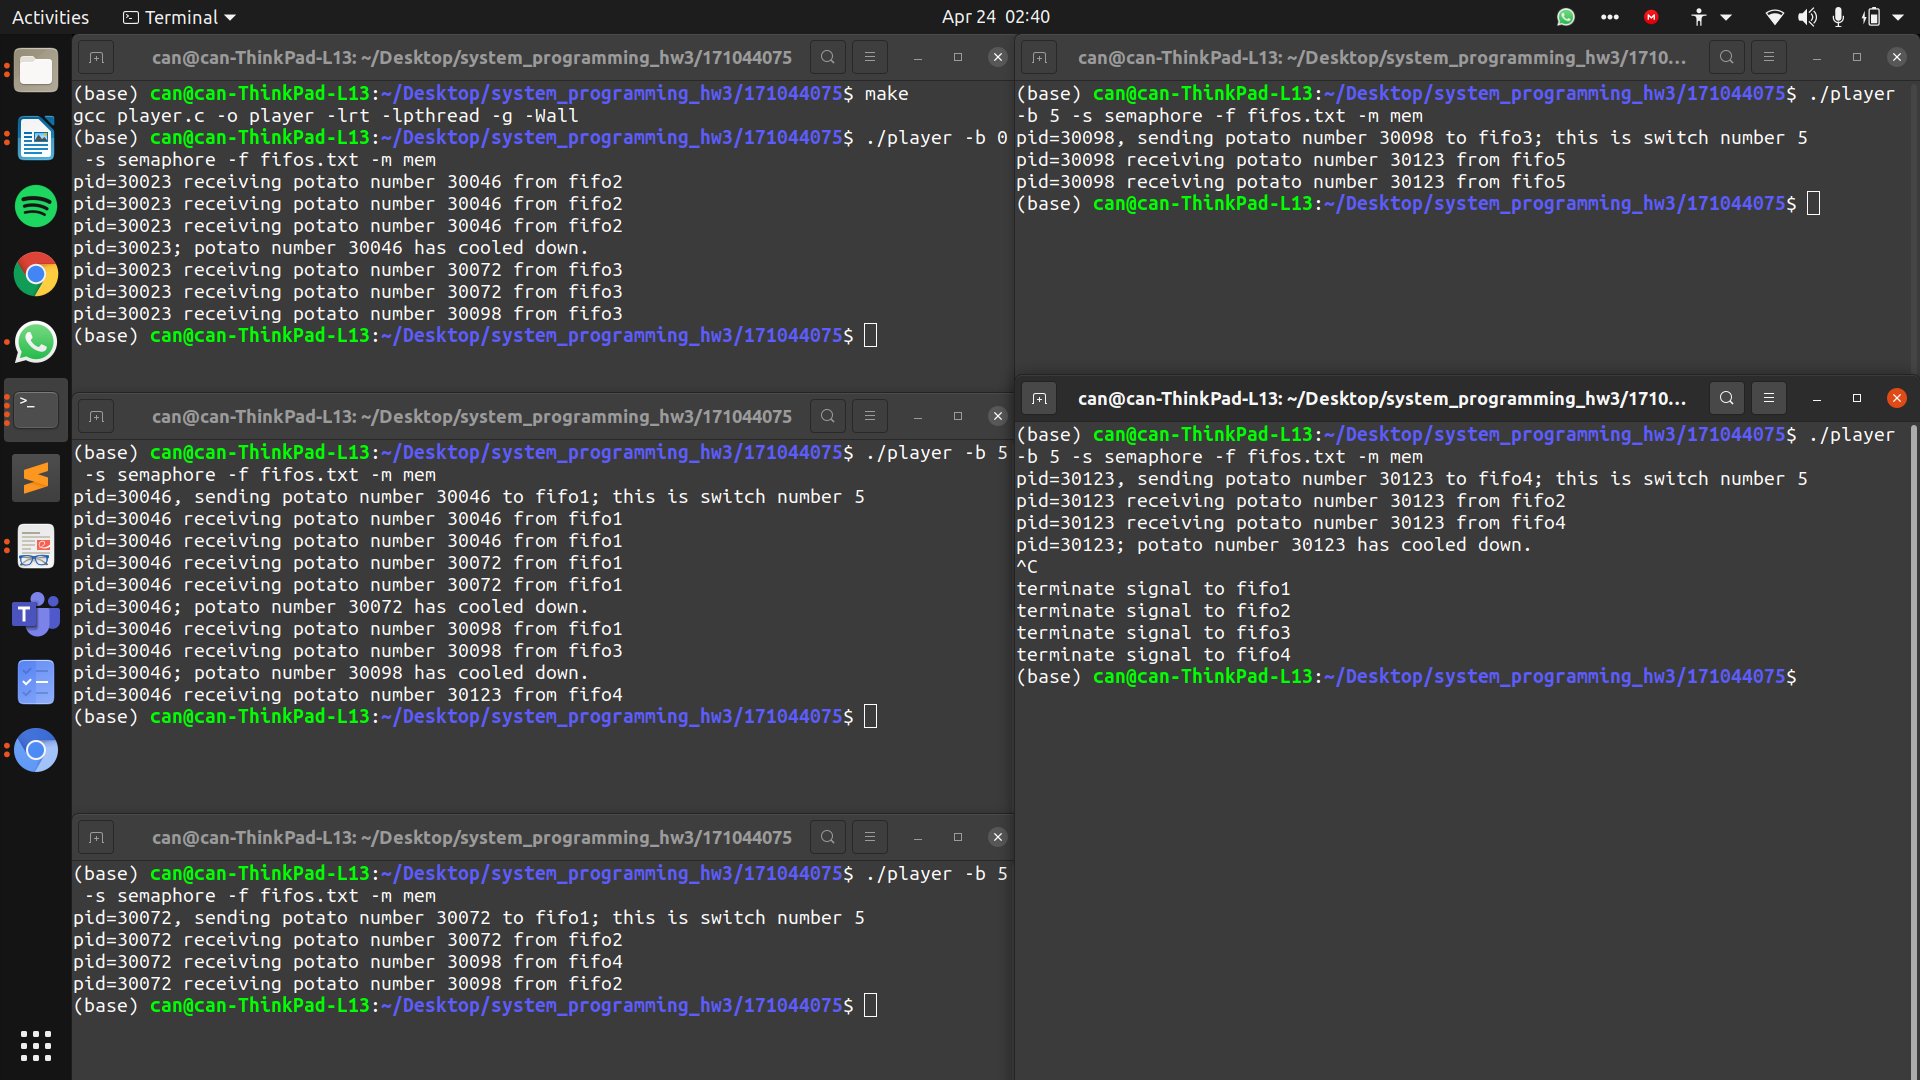
\includegraphics[width=120mm]{2.png}
	\caption{Running of the program \label{overflow}}
\end{figure}



{\color{red}\large\textbf {Which requirements I achieved and which I have failed:}}\newline\\
\phantom{beta}Every requirements are done! I tried to pay attention to everything written in pdf as much as I could.\newline\\
\end{document}

